\section{Introduction}
\label{sec:intro}

Some properties of natural and engineered materials can be analyzed by
treating them as two dimensional (2D) layers. As illustrated by the
examples below, the structure within each layer is often self-
similar~\cite{2012arXiv1204.6389G} spanning multiple scales; generally
aperiodic and quasi-uniform within any one scale; and consists of a
few repeated motifs appearing in disordered arrangements. Each layer
is not necessarily planar, i.e., it consists of multiple, inter-
constraining planar (genus 0) monolayers. Furthermore, a layer is
often  either \vemph{isostatic or underconstrained, not self-
stressed} (See Section \ref{sec:prelim} for definitions). These
properties are consistent with a self-assembled 2D structure that
minimizes mass, optimally distributes external stresses and itself
participates in the assembly of diverse and multifunctional, larger 2D
structures.

\noindent
\textbf{Note on Scope:} In this manuscript we only study finite 2D structures.
\dfn{Self-similarity} refers to the result of finitely many levels of hierarchy
or subdivision in an iterated scheme to generate self-similar structures.

\begin{figure*}\centering
% \begin{subfigure}{.31\linewidth}\centering
%   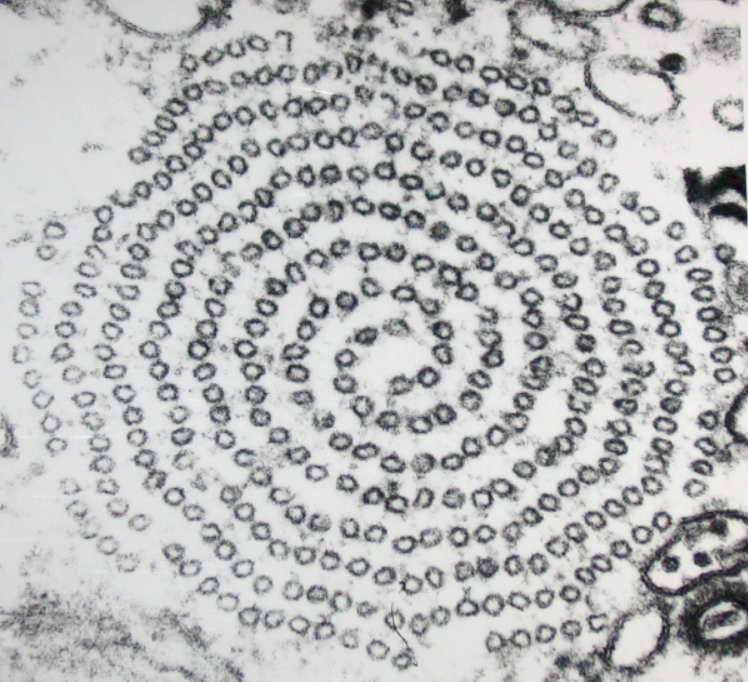
\includegraphics[width=\linewidth]{img/Axopodium_Mikrotubuli}
%   \caption{Cross section of a Heliozoa's psuedopod, formed by a spiral structure of microtubules.}
%   % https://de.wikipedia.org/wiki/Mikrotubulus#mediaviewer/File:Axopodium_Mikrotubuli.jpg
%   \label{fig:material_examples:microtubule}
% \end{subfigure}\hfill
% \begin{subfigure}{.31\linewidth}\centering
%   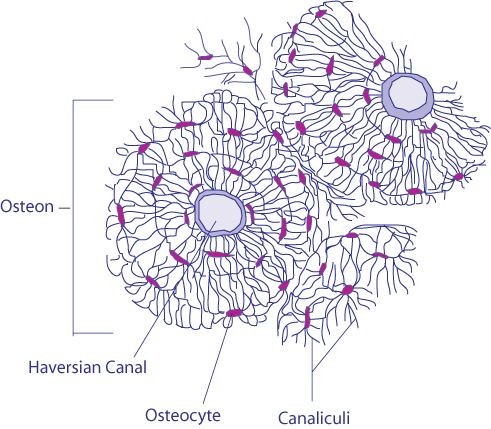
\includegraphics[width=\linewidth]{img/Transverse_Section_Of_Bone}
%   \caption{Cross section of an osteon (the fundamental unit of compact bone) exhibiting its hierarchical structure.}
%   % https://en.wikipedia.org/wiki/Osteon#mediaviewer/File:Transverse_Section_Of_Bone.png
%   \label{fig:material_examples:osteon}
% \end{subfigure}\hfill
\begin{subfigure}{.28\linewidth}\centering
  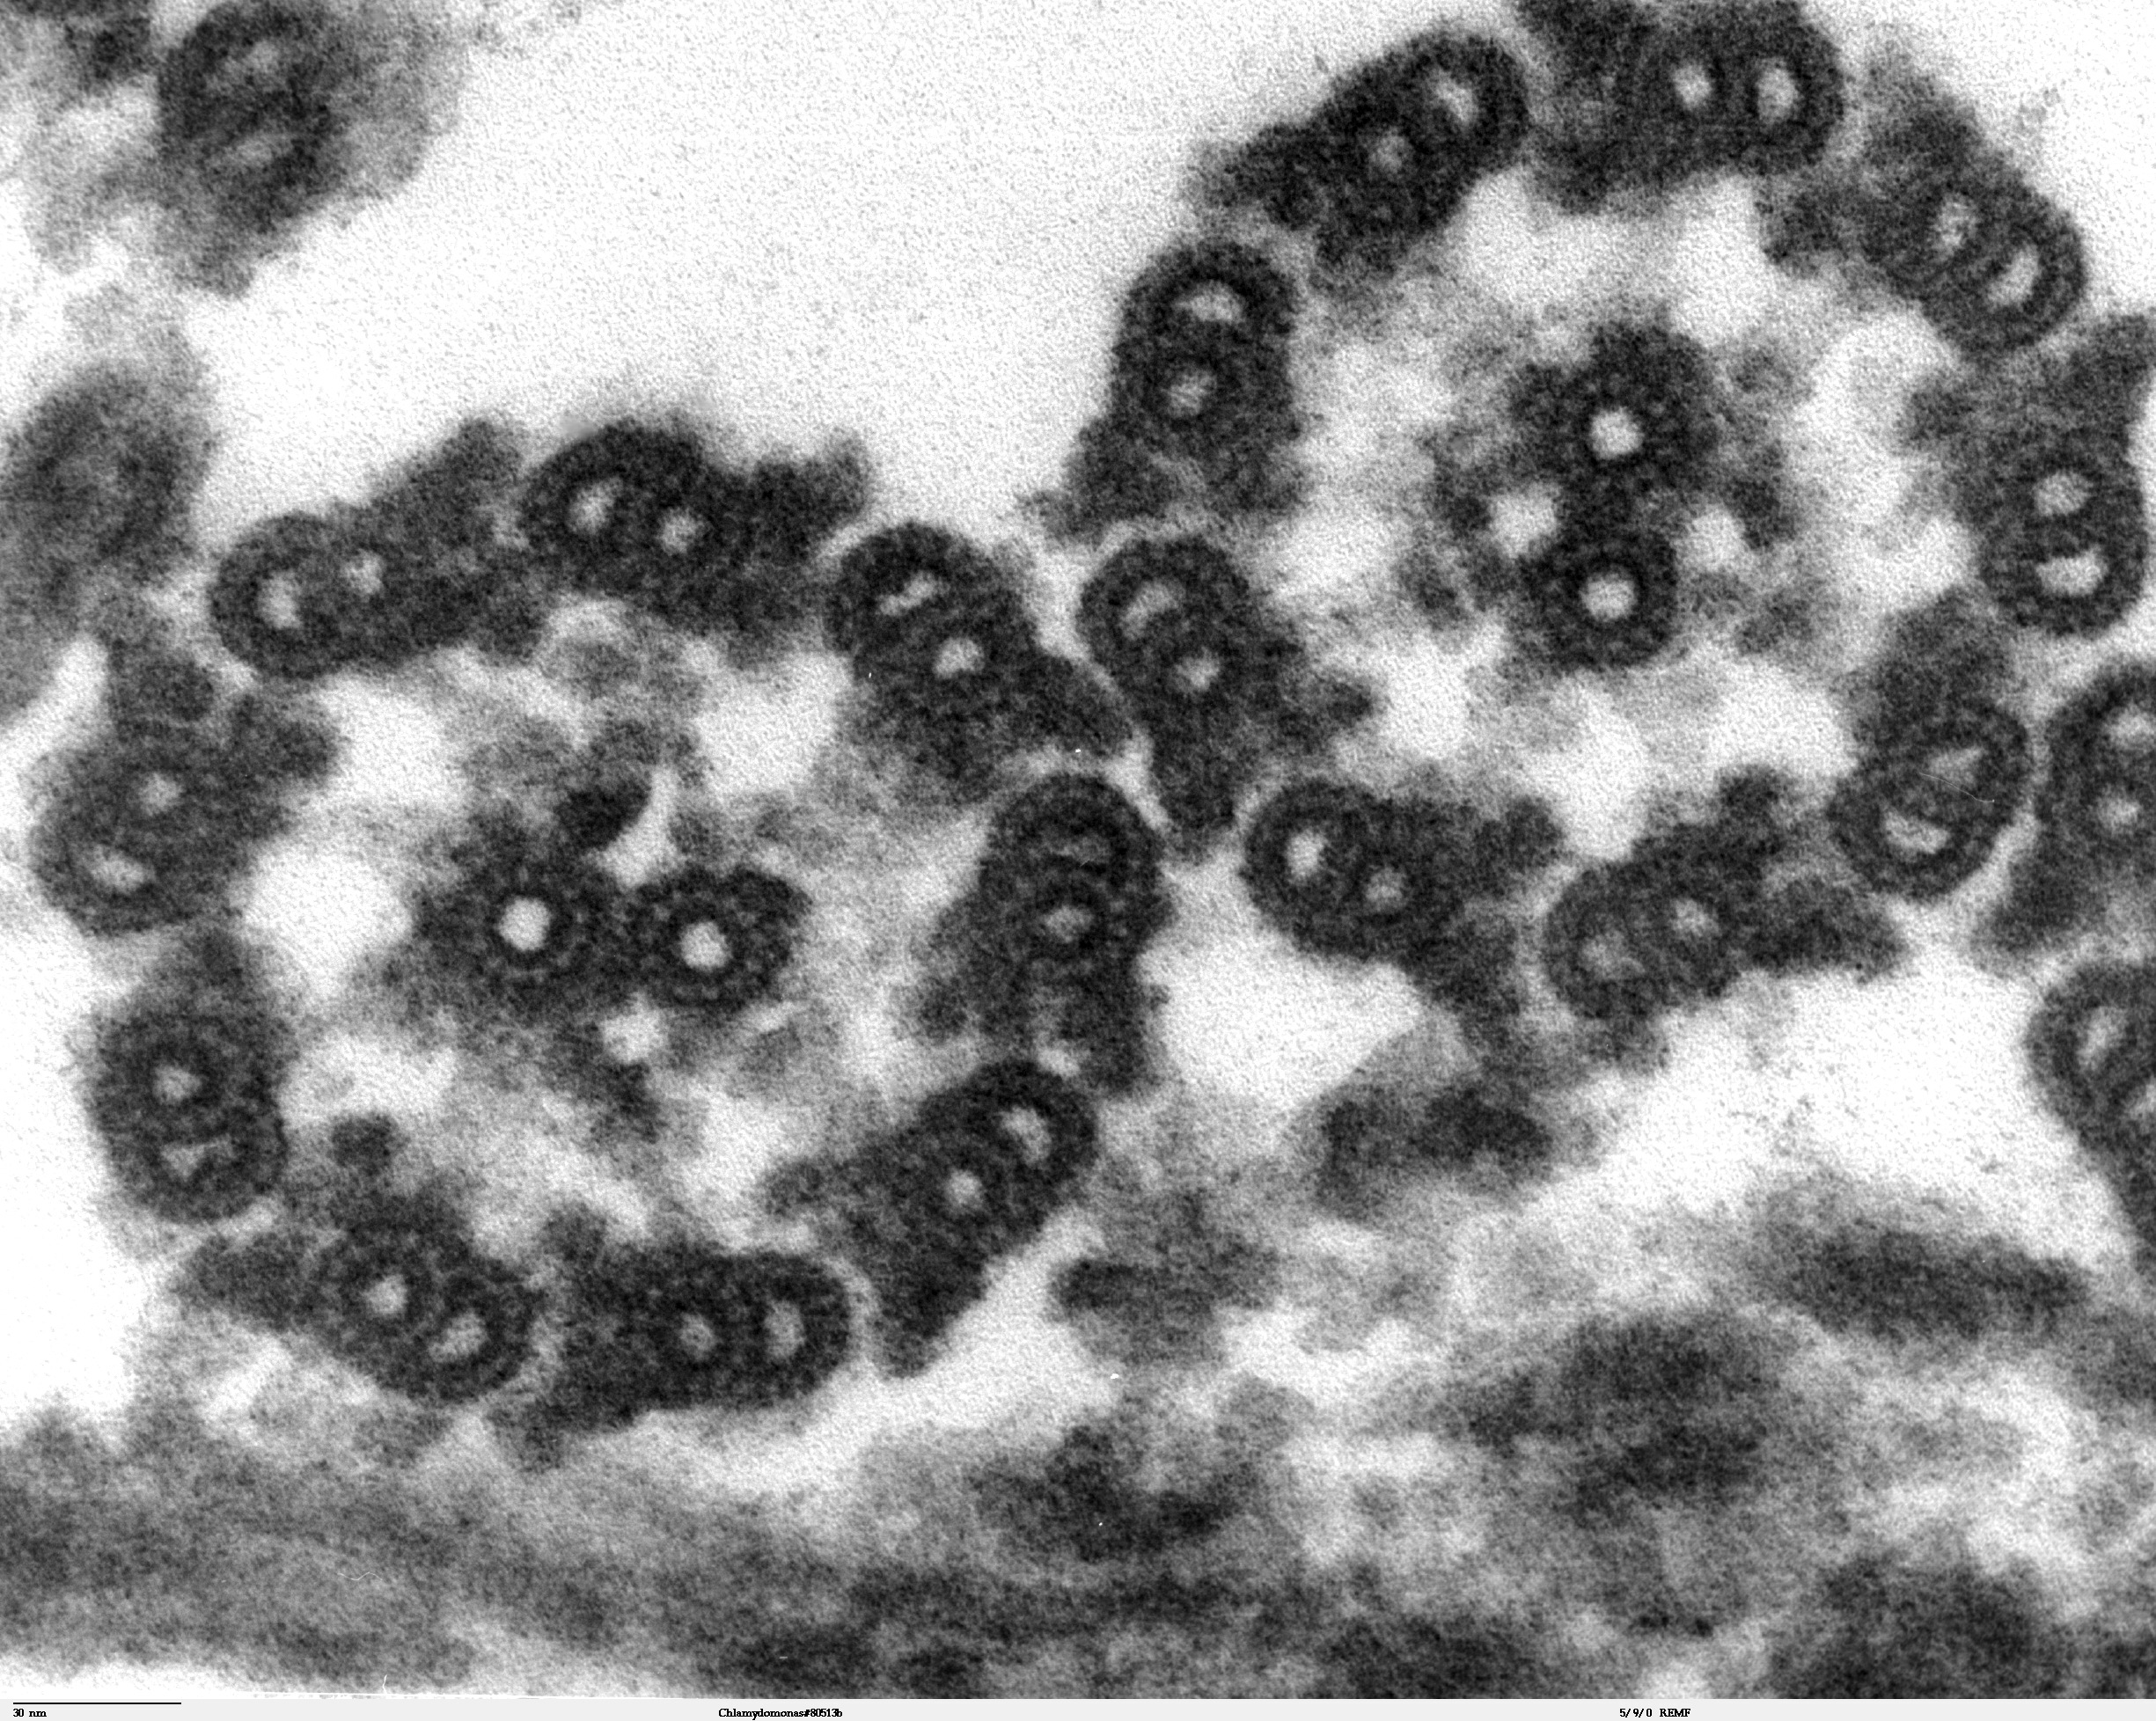
\includegraphics[width=\linewidth]{img/Chlamydomonas_TEM_17}
  \caption{Cross section of the Chlamydomonas algae axoneme, a cilia composed of microtubules~\cite{wikimediacommons2007cilia}.}
  \label{fig:material_examples:microtubule}
\end{subfigure}\hfill
\begin{subfigure}{.40\linewidth}\centering
  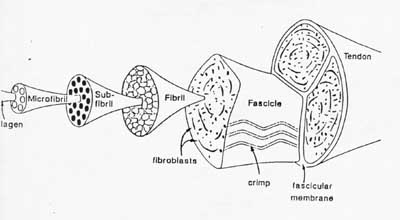
\includegraphics[width=\linewidth]{img/ligten2}
  \caption{Cross section of a tendon displaying the hierarchical structure~\cite{lecture_biosolid_mechanics}.}
  \label{fig:material_examples:tendon}
\end{subfigure}\hfill
\begin{subfigure}{.30\linewidth}\centering
  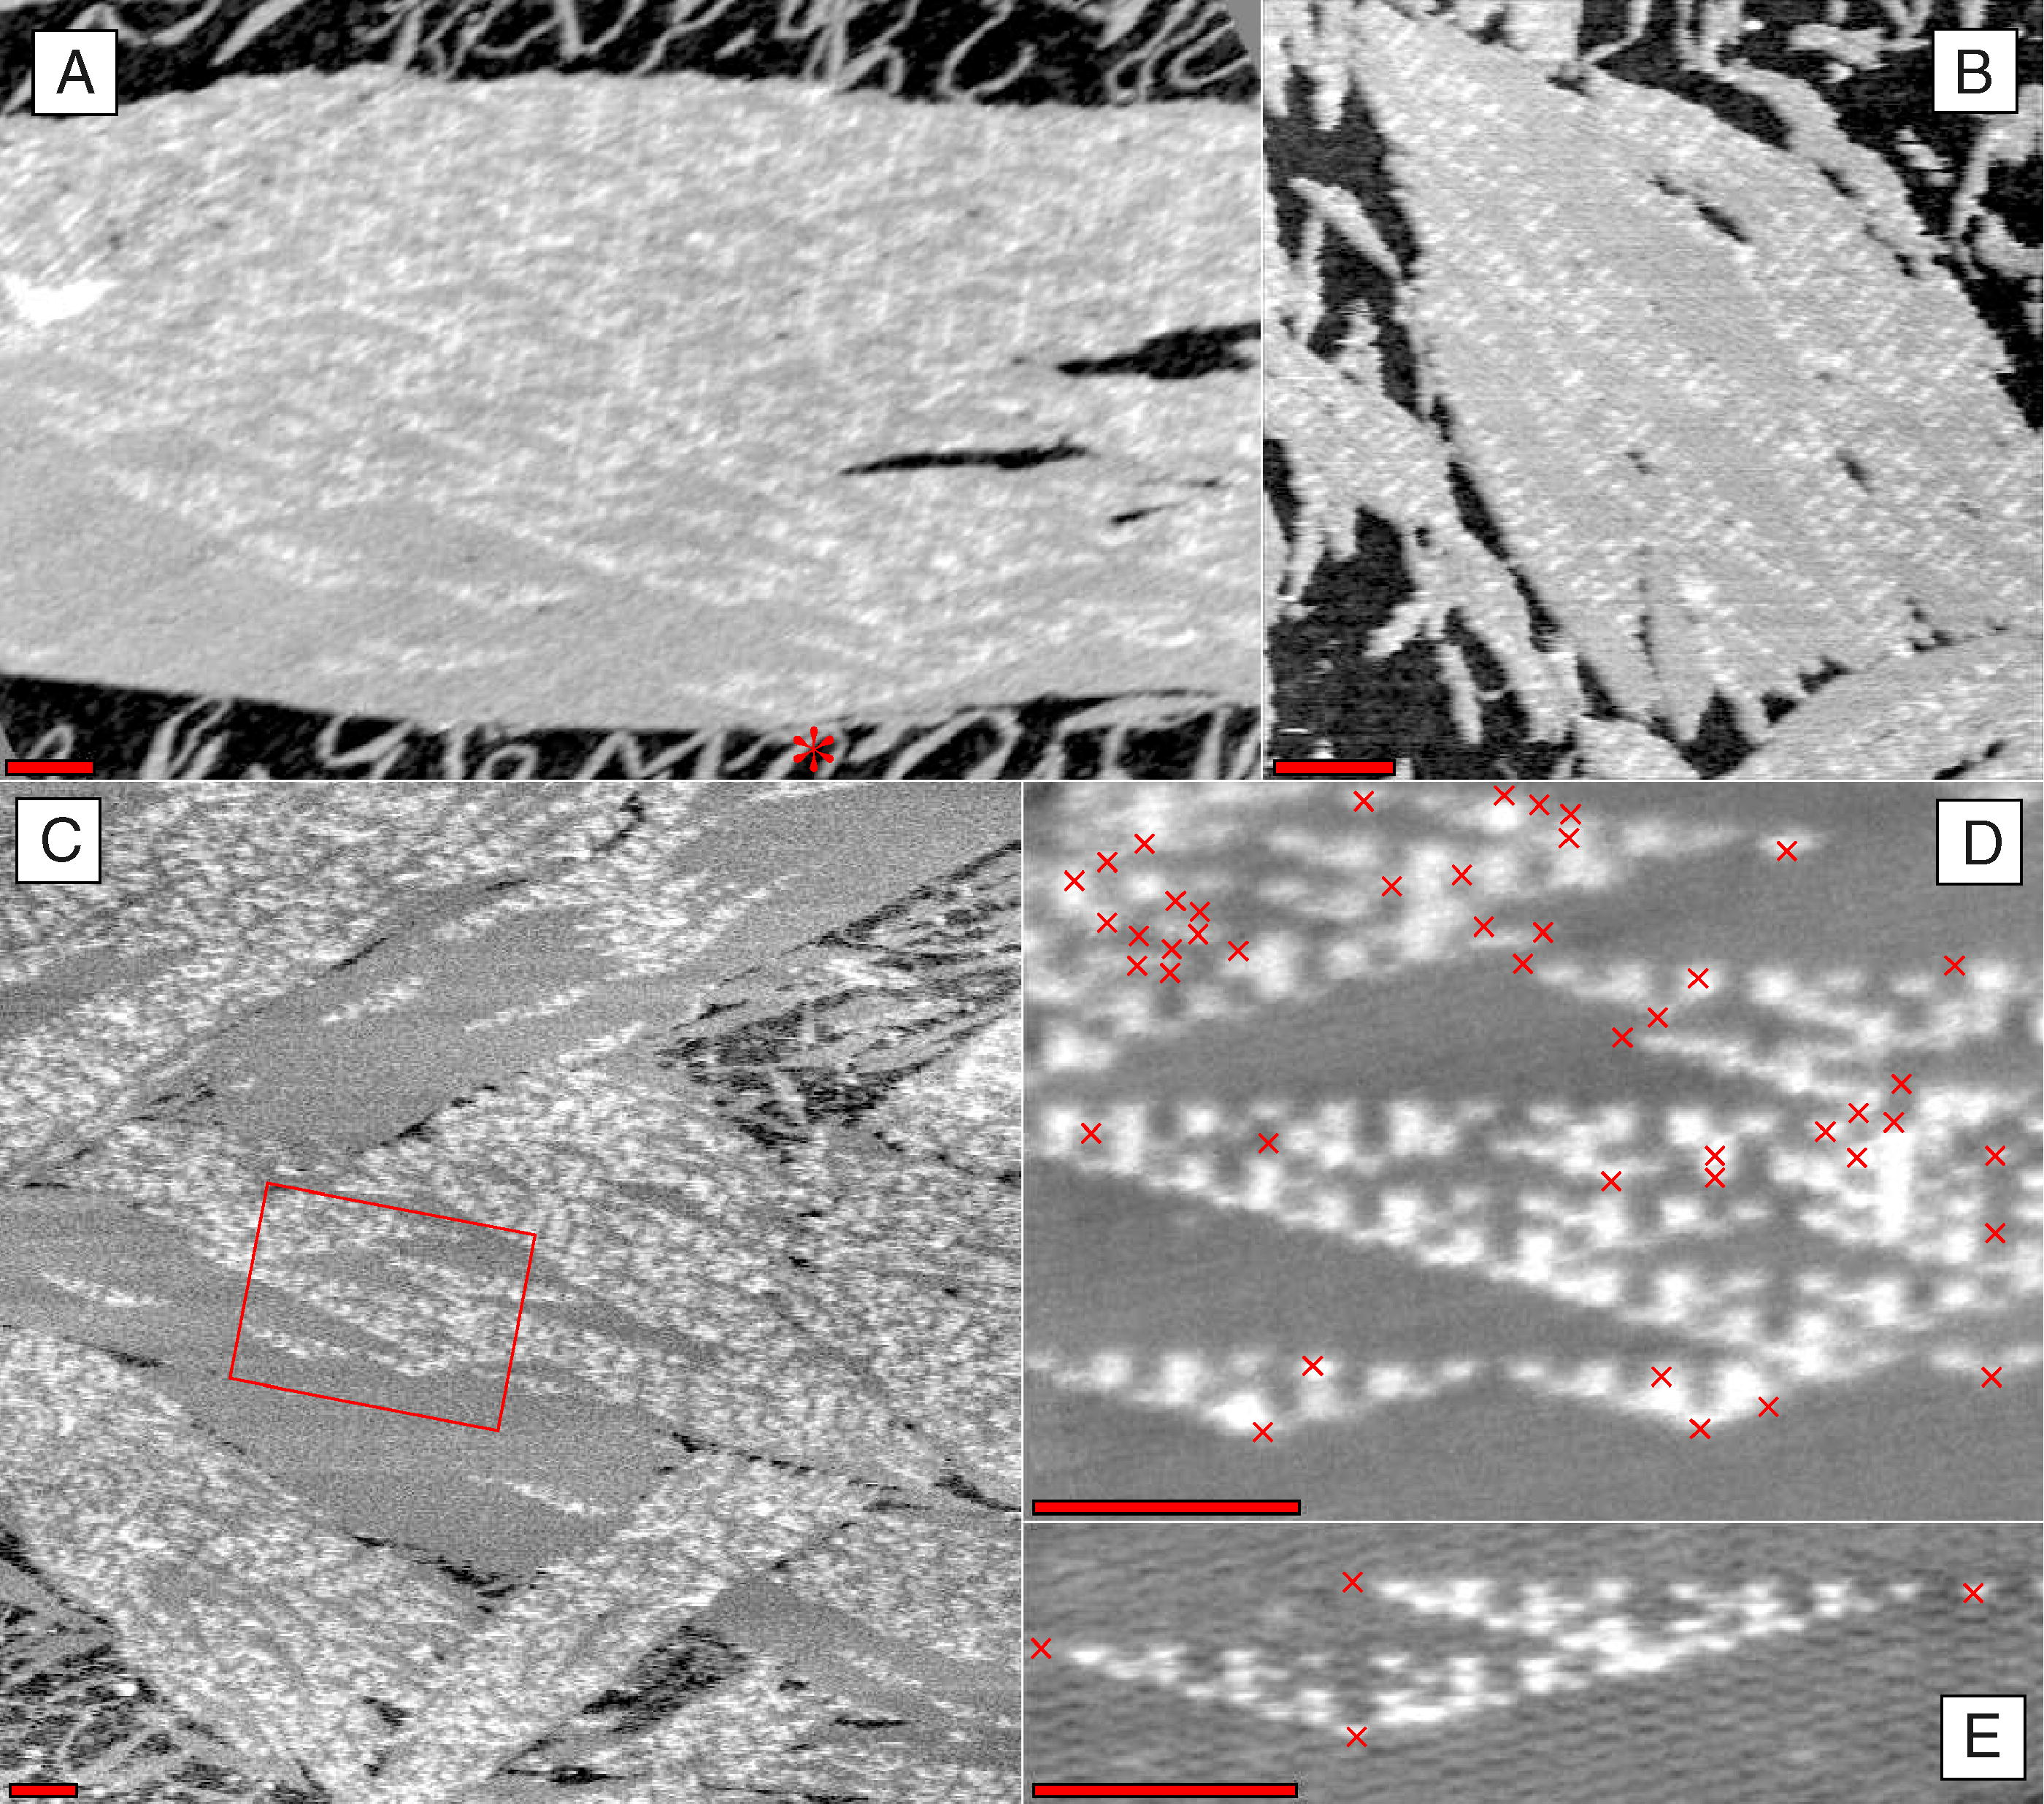
\includegraphics[width=\linewidth]{img/Rothemund-DNA-SierpinskiGasket}
  \caption{A DNA array exhibiting the Sierpinski triangle~\cite{wikimediacommons2007dna}.}
  \label{fig:material_examples:sierpinski}
\end{subfigure}
\caption{}\label{fig:material_examples}
\end{figure*}


Examples of such materials (See Figure \ref{fig:material_examples})
include:
%
\begin{enumerate}
    \item \label{materialexample1} Cross-sections of microtubule structures~\cite{microtubule_necklace} (Figure \ref{fig:material_examples:microtubule}) e.g., in ciliary membranes and transitions~\cite{microtubule_cilia}.

    \item \label{materialexample2} Cross-sections of organic tissue with hierarchical structure, e.g. compact bone and tendon (Figure \ref{fig:material_examples:tendon}).

    \item \label{materialexample3} Crosslinked cellulose or collagen microfibril monolayers e.g., in cell-walls~\cite{wikimediacommons2010afm}~\cite{wikimediacommons2007plant}, as well as crosslinked actin filaments in the cytoskeleton matrix. See Section \ref{sec:pinnedline}.

    \item \label{materialexample4} More recent, engineered examples, including disordered
    graphene layers~\cite{Graphene1}~\cite{Graphene2} sometimes
    reinforced by microfibrils; and DNA assemblies including a recent
    Sierpinski gasket~\cite{self_assembly_sierpinski}, bringing other
    self-similar structures~\cite{wikimediacommons2012subdivision} within reach.

    \item \label{materialexample5} Silica bi-layers~\cite{silica_bilayers}, glass~\cite{sructure_of_2d_glass}, and
    materials that behave like assemblies of 2D particles under
    non-overlap constraints, i.e, like jammed disks on the plane~\cite{jammed_disks}. See Section \ref{sec:bodypin}.
\end{enumerate}
%
In order to study structural and mechanical properties
of a material layer, it is natural to model a material layer as a solution or
realization of a geometric constraint system of appropriate types of geometric
primitives, under metric or algebraic constraints. Such 2D
\dfn{qusecs} (quasi-uniform or self-similar constraint systems, defined
formally in Section \ref{sec:prelim}) can be
used to understand or design material layers (their solutions) with
desired properties.
%
\subsection{Previous Work on Relevant 2D Geometric Constraint Systems}
We now briefly survey existing techniques for studying 2D
qusecs,  many of which are \dfn{bar-joint} systems
(Examples 1, 2 above, see Sections \ref{sec:prelim}, \ref{sec:DRP}, \ref{sec:recomb}),
\dfn{body-hyperpin} systems (Example 4,5, see Section
\ref{sec:bodypin}) or \dfn{pinned-line incidence} systems (Example
3, see Section \ref{sec:pinnedline}). The limitations of these
techniques directly motivate the contributions of this paper.

\medskip\noindent
\header{(i) Finding (vertex)-maximal generically rigid subsystems}
Fast, graph-based algorithms exist (pebble-game \cite{Jacobs:1997:PG,lee2005finding}), for locating all maximal,
\dfn{generically rigid} subsystems (defined formally in Section
\ref{sec:prelim}). When the input itself is rigid, these
algorithms do nothing, i.e., compute the identity function.

However, both for self-similar or just aperiodic 2D qusecs, it is
imperative to recursively decompose rigid systems into their rigid
subsystems, down to the level of geometric primitives, in order to
understand or design properties at all scales, such as (formally
defined in Section \ref{sec:prelim}) \dfn{rigidity}, \dfn{flexes},
distribution of \dfn{external stresses}, boundary conditions for
\dfn{isostaticity}, as well as behavior under constraint variations.

\medskip\noindent
\header{(ii) Optimal Recursive Decomposition (DR-planning).}
Recursive decomposition of geometric constraint systems has been
formalized \cite{hoffman2001decompositionI,hoffman2001decompositionII} and well-studied \cite{jermann2006decomposition,sitharam2005combinatorial} as the
\dfn {Decomposition-Recombination (DR)-planning} problem, defined formally in
Section \ref{sec:prelim}. For the above-
mentioned classes of 2D qusecs, generic rigidity is a combinatorial
property and hence each level of the decomposition should, in
principle, be achievable by a graph-based algorithm as in (1), without
involving geometric information in the constraint system. Since many
such decompositions can exist for a given constraint system, criteria
defining desirable or optimal DR-plans and DR-planning algorithms were
given in \cite{hoffman2001decompositionI}. An \dfn{optimal DR-plan} is one that minimizes
the \dfn{size} (defined formally in Section \ref{sec:prelim}, i.e.,
the maximum number of child subsystems of any parent system.
Being exponential the size, the complexity of solving the parent
constraint system from the solutions of the child systems, is overwhelmingly
dominated by it.

However, for general 2D qusecs that could be overconstrained, even
when restricted to bar-joint systems, the optimal DR-planning problem
was shown to be NP-hard \cite{lomonosov2004graph}.

\medskip\noindent
\header{(iii) DR-plans for special classes and with other
criteria.}
For a special class of 2D qusecs, namely \dfn{tree-decomposable}
systems  \cite{fudos1997graph,owen1991algebraic,joan-arinyo2004revisiting}  common in computer aided mechanical design, (which
includes ruler-and-compass and Henneberg-I constructible systems), all
DR-plans turn out to be optimal. This satisfies the so-called \dfn
{Church-Rosser} criterion, leading to highly efficient DR-planning
algorithms. For general 2D qusecs, alternate criteria were suggested
such as \dfn{cluster minimality} requiring parent systems to be
composed of a minimal set of at least 2 rigid proper subsystems (i.e.,
no proper subset forms a rigid system); and \dfn{proper maximality},
requiring child subsystems to be maximal rigid proper subsystems of
the parent system. See Section \ref{sec:prelim} for formal definitions.

While polynomial time algorithms were given \cite{hoffman2001decompositionI} to generate DR-
plans meeting the cluster minimality criterion, no such algorithm is
known for the latter criterion.


\medskip\noindent
\header{(iv) Optimal Recombination and Solution Space Navigation.}
For the entire DR-plan, finding all desired solutions is barely
tractable even if recombination of solved subsystems is easy for each
indecomposable parent system in the DR-plan. This is because even for
the simplest, highly decomposable systems with small DR-plans, the
problem of finding even a single solution to the input system at the
root of the DR-plan is NP-hard  \cite{saxe1979embeddability}
and there is a combinatorial explosion of solutions \cite{borcea2004number}. Typically, however, the desired
solution has a given orientation type, in which case, the crux of the
difficulty is concentrated in the algebraic complexity of
(re)combining child system solutions, to give a solution to the parent
system at any given level of the DR-plan. For fairly general 3D
constraint systems, there are algorithms with formal guarantees that
uncover underlying matroids to combinatorially obtain an optimal
parameterization to minimize the algebraic complexity of the
indecomposable parent (sub)systems that occur in the DR-plan
\cite{sitharam2010optimized,sitharam2006well,sitharam2010reconciling}, provided the DR-plan meets some of the
abovementioned criteria.

However, the generality of these algorithms trades-off against
efficiency, and despite the optimization, the best algorithms can
still take exponential time in the number of child subsystems (which
can be arbitrarily large even for optimal DR-plans) in order to
guarantee all solutions of a given orientation type, even for a single
(sub)system in a DR-plan. They are prohibitively slow in practice. We
note that, utilizing the DR-plan and optimal recombination as a
principled basis, high performance heuristics and software exists
\cite{sitharam2006solution} to tame combinatorial explosion via user intervention.


\medskip\noindent
\header{(v) Configuration Spaces of Underconstrained Systems.}
For underconstrained 2D bar-joint and body-hyperpin qusecs obtained
from various subclasses of tree-decomposable systems, algorithms have
been developed to complete them into isostatic systems
\cite{joan-arinyo2003transforming,sitharam2005combinatorial,gao2006ctree,sitharam2010convex} and to find paths within the connected components
\cite{sitharam2011cayleyI,hidalgo2011reachability} of standard Cartesian configuration spaces.
Most of the
algorithms with formal guarantees leverage Cayley configuration space
theory \cite{sitharam2010convex,sitharam2011cayleyI,sitharam2011cayleyII} to characterize subclasses of graphs and
additional constraints that control combinatorial explosion, and
provide faithful bijective representation of connected components and
paths. These algorithms have decreasing efficiency as the subclass of
systems gets bigger, with highest efficiency for underlying partial
2-tree graphs (alternately called, tree-width 2, series-parallel, $K_4$
minor avoiding), moderate efficiency for 1 degree- of-freedom (dof)
graphs with low Cayley complexity (which include common linkages such
as the Strandbeest, Limacon and Cardioid), and decreased efficiency
for general 1-dof tree-decomposable graphs. While software suites
exist  \cite{keycurriculum1995geometer,porta2014open,siemens1999d,todd2007geometry}, no such formal algorithms and guarantees are known
for non-tree-decomposable systems.
%
\subsection{Contributions and Organization}
\label{sec:cont}

The contributions of this paper are the following.
\begin{itemize}
  \item In Section \ref{sec:DRP}, we navigate the NP-hardness barrier mentioned in (2) above,
  for finding optimal DR-plans by defining a so-called \dfn{canonical}
  DR-plan and showing a strong Church-Rosser property: \vemph{all
  canonical DR-plans for isostatic or underconstrained 2D qusecs are
  optimal}.

  \item Also in Section \ref{sec:DRP}, we give an efficient (\candrpcomplexity) algorithm to find a canonical
  (and hence optimal) DR-plan for all 3 types of 2D qusecs mentioned
  above (Sections \ref{sec:DRP}, \ref{sec:bodypin}, and
  \ref{sec:pinnedline}). The canonical DR-plan elucidates the essence
  of the NP-hardness of finding optimal DR-plans for over-constrained
  systems. Futhermore, our optimal/canonical DR-plan satisfies desirable properties such as Cluster Minimality previously studied \cite{hoffman2001decompositionI}.

  \item In Section \ref{sec:recomb}, we give a method to deal with the
  algebraic complexity of recombining the realizations or solutions of
  child subsystems into a solution of the parent system
  \cite{sitharam2010optimized,sitharam2006well,sitharam2010reconciling}
  Specifically, we define the problem of minimally modifying the
  indecomposable recombination system so that it becomes decomposable
  via a small DR-plan and yet preserves the original solutions in an
  efficiently searchable manner. In Section \ref{sec:table}, we show formal connection to well
  known problems such as optimal completion of underconstrained
  systems
  \cite{joan-arinyo2003transforming,sitharam2005combinatorial,gao2006ctree}
  and to find paths within the connected components. When the
  modifications are bounded, we obtain new, efficient algorithms for
  realizing both isostatic and underconstrained qusecs by leveraging
  recent results about Cayley parameters in
  \cite{sitharam2010convex,sitharam2011cayleyI,sitharam2011cayleyII} (see Sections \ref{sec:2-tree-reduction} and \ref{sec:tdecomp}).

  \item In Section \ref{sec:bodypin} and \ref{sec:pinnedline}, we
  briefly describe applications of the above techniques to modeling,
  analyzing, and designing specific properties in 2D material
  layers~\cite{Jackson2008bodypin}. For Examples
  \ref{materialexample1}, \ref{materialexample2} (achieving
  isostaticity, distribution of stresses in self-similar, bar-joint
  systems); Example \ref{materialexample3} (canonical and optimal DR-
  plans for pinned line incidence systems
  \cite{sitharam2014incidence}) and Examples \ref{materialexample4},
  \ref{materialexample5} (boundary-conditions for achieving various
  desired properties of body-hyperpin systems).

  \item We intend to make software implementation and videos available
  upon request and publicly available for the final version of the
  paper.
\end{itemize}

\noindent
\note All proofs appear in the Appendix (submitted an a permitted attachment via EasyChair).
